\documentclass[10pt]{beamer}
% Class options include: notes, notesonly, handout, trans,
%                        hidesubsections, shadesubsections,
%                        inrow, blue, red, grey, brown

% Theme for beamer presentation.
\usepackage{beamerthemesplit} 
%\usepackage{times}
\usepackage{anysize}
\usepackage{fancyhdr}
\usepackage{graphicx}
\usepackage{pdfpages}
\usepackage{amsmath}
\usepackage{amssymb}
\usepackage{pgfplots}
% Other themes include: beamerthemebars, beamerthemelined, 
%                       beamerthemetree, beamerthemetreebars  

\title{The Fast Multipole Algorithm vs. the Particle Mesh Ewald Method}    % Enter your title between curly braces
\author{Joshua Nelson, u4850020}                 % Enter your name between curly braces
\institute{COMP3006 - Research Project}      % Enter your institute name between curly braces
\date{\today}                    % Enter the date or \today between curly braces

\usetheme{PaloAlto}
\usecolortheme{beaver}

\newcommand{\bcen}{\begin{center}}
\newcommand{\ecen}{\end{center}}

\addtobeamertemplate{frametitle}{
   \let\insertframetitle\insertsectionhead}{}

\begin{document}
%---------------------TITLE PAGE---------------------------
% Creates title page of slide show using above information
\begin{frame}
  \titlepage
\end{frame}
\note{} % Add notes to yourself that will be displayed when
        % typeset with the notes or notesonly class options
%---------------------PROBLEM DESCR------------------------
\section{The N body problem}
\begin{frame}
\frametitle{Statement of the problem}
\framesubtitle{Statement of the problem}
\bcen
\large \emph{Given $N$ bodies that all interact with each other in some way, how do we efficiently calculate the effect each body has on every other body?}
\ecen
\end{frame}
\note{Electrostatics, molecular dynamics, astrophysics examples. Interactions are a function of distance}

\begin{frame}
\frametitle{History of the N body problem}
\framesubtitle{History}
\begin{itemize}
\item<1-> First formally specified by Isaac Newton
\item<2-> No exact formula solution
\item<3-> Approximation methods devised
\end{itemize}
\end{frame}
\note{Newton showed a formula for N=2, Poincare showed there was no solution for $N > 3$.}

\begin{frame}
\frametitle{Applications of the N body problem}
\framesubtitle{Applications}
\bcen \includegraphics<1>[width=7.5cm,bb= 0 0 2048 1536,clip]{millenium_run.jpg} \ecen
\bcen \includegraphics<2>[width=7.5cm,bb= 0 0 1589 1609,clip]{plasma.jpg} \ecen
\bcen \includegraphics<3>[width=7.5cm,bb= 0 0 1144 936,clip]{molecule.jpg} \ecen
\end{frame}
\note{Millenium run - simulates the universe on a grand scale, from the formation to it's current state and beyond. Bodies = planets and galaxies. Plasma - plasma can be simulated as a collection of particles interacting. Molecular dynamics - the problem of simulating a molecule is essentially the N body problem (electrostatic)}

\section{The basic solution}
\begin{frame}
\frametitle{The basic solution}
\framesubtitle{Algorithm}
\begin{itemize}
\item<1-> Say that a particle at position $r_i$ with charge $q_i$ gives a potential $Q$ at a particle $r_j$ with charge $q_j$ according to the formula
\bcen
\[
Q = \frac{q_i * q_j}{|r_i-r_j|}
\]
\ecen
\item<2-> For each particle pair, calculate the the interaction according to the above formula
\item<3-> Use the potential at each particle to calculate the force, and move the particle according to this force.
\item<4-> Order $O(n^2)$ complexity.
\end{itemize}
\end{frame}

\section{The Fast Multipole Algorithm}
\begin{frame}
\frametitle{The Fast Multipole Algorithm}
\framesubtitle{Key components to the Fast Multipole Algorithm}
\bcen Key components to the Fast Multipole Algorithm \ecen
\begin{itemize}
\item<1-> The Mesh
\item<2-> Multipole Expansions
\end{itemize}
\end{frame}

\begin{frame}
\frametitle{The Fast Multipole Algorithm}
\framesubtitle{The Mesh}
\bcen The Particle Mesh \ecen
\bcen \includegraphics<1>[width=0.35\textwidth]{fma_mesh.pdf} \ecen
\end{frame}
\note{We split the simulation cell into a mesh, dividing it in two multiple times to create this tree structure of coarser to finer meshes.}


\begin{frame}
\frametitle{The Fast Multipole Algorithm}
\framesubtitle{The Mesh}
\bcen Well separated cells \ecen
\bcen \includegraphics<1>[width=0.35\textwidth]{wellsep.pdf} \ecen
\end{frame}
\note{We calculate interactions in the same way as the basic algorithm for cells that are not well separated, and use Local Expansions if they are well separated}



\begin{frame}
\frametitle{The Fast Multipole Algorithm}
\framesubtitle{Expansions}
\begin{itemize}
\item<1-> Multipole Expansions: A series, centered on a particular cell, which can approximate the potential from the cell's particles near that cell
\item<2-> Local Expansions: A series, centered on a particular cell, formed from a Multipole Expansion, which approximates the potential from within the cell at some distance away from that cell.
\end{itemize}
\end{frame}

\begin{frame}
\frametitle{The Fast Multipole Algorithm}
\framesubtitle{Aglorithm}
\begin{itemize}
\item<1-> Form Multipole Expansions at the lowest mesh level
\item<2-> Translate them to their parent's cells, combining the four children by summing them to form the parent's Multipole Expansion
\item<3-> Repeat the above for each level
\item<4-> At the highest level, from the Multipole Expansion, form a Local Expansion.
\item<5-> Translate this to children nodes, repeat to the lowest mesh level.
\end{itemize}
\note{Going up and going down the tree again. Go up with multipole, down with local.}
\end{frame}

\section{Particle Mesh Ewald Method}
\begin{frame}
\frametitle{Particle Mesh Ewald Method}
\framesubtitle{Basic structure of the Particle Mesh Ewald Method}
\bcen Basic structure of the Particle Mesh Ewald Method \ecen
\begin{itemize}
\item<1-> Interpolate particles to a grid
\bcen \includegraphics<1>[width=0.75\textwidth]{Qarray.jpg} \ecen
\item<2-> Perform a fourier transformation on the grid
\item<3-> Calculate long range potential in reciprocal space using this grid
\item<4-> Return to real space using another fourier transformation
\item<5-> Calculate in real space directly for near particles, and use interpolated grid values for the long range potential.
\end{itemize}
\end{frame}

\begin{frame}
\frametitle{Particle Mesh Ewald Method}
\framesubtitle{Characteristics of the Particle Mesh Ewald Method}
\bcen Characteristics of the Particle Mesh Ewald Method \ecen
\begin{itemize}
\item<1-> Complexity of $O(n\text{log}(n))$
\item<2-> Fourier transformation technique leads to Periodic Boundary Conditions
\bcen \includegraphics<2>[width=0.75\textwidth]{pbc.pdf} \ecen
\end{itemize}
\end{frame}
\note{$O(n\text{log}(n))$ comes from the FFT part}

\section{Results}
\begin{frame}
\frametitle{Basic Algorithm complexity}
\framesubtitle{Basic Algorithm}
\bcen 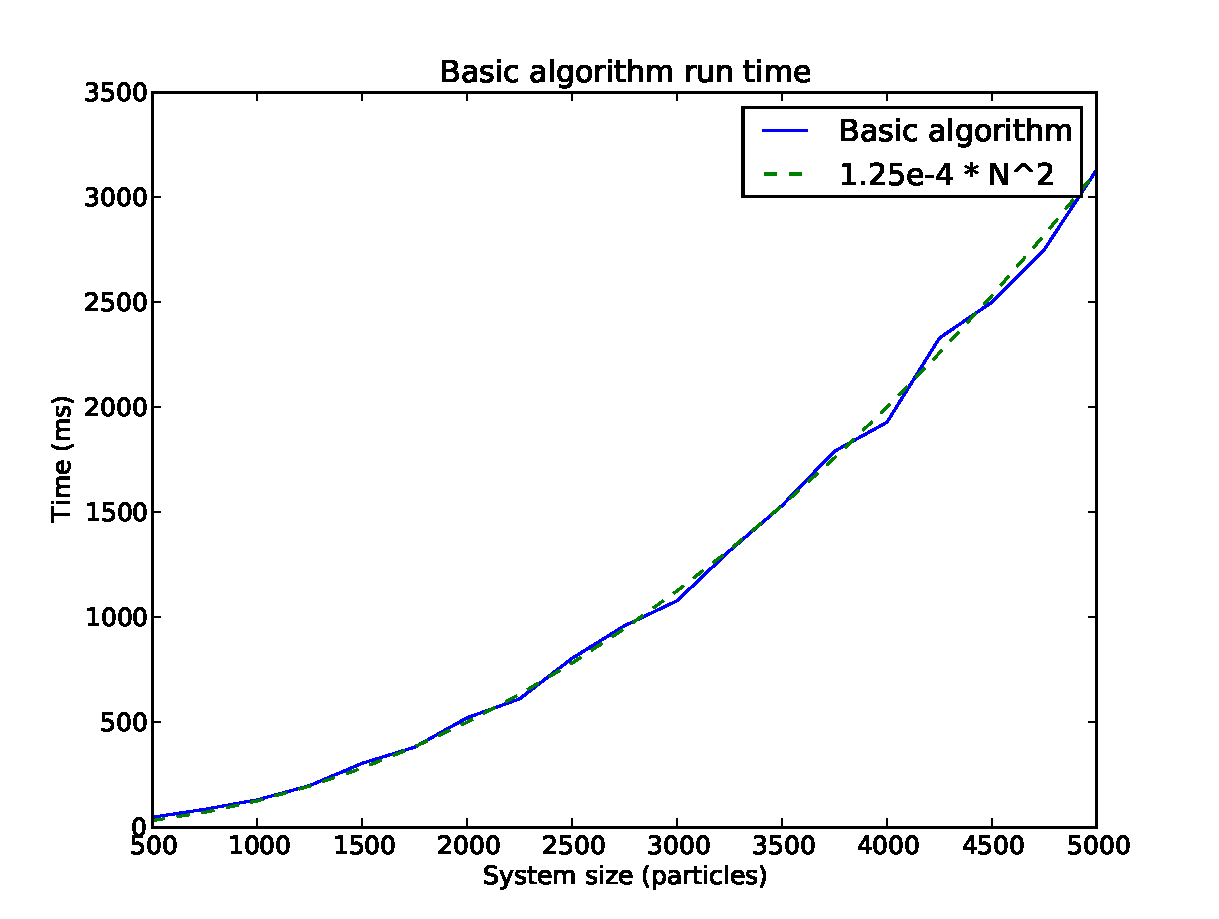
\includegraphics[width=\textwidth]{basic_algo_complex.pdf} \ecen
\end{frame}

\begin{frame}
\framesubtitle{Fast Multipole Algorithm}
\frametitle{Fast Multipole Algorithm complexity}
\bcen 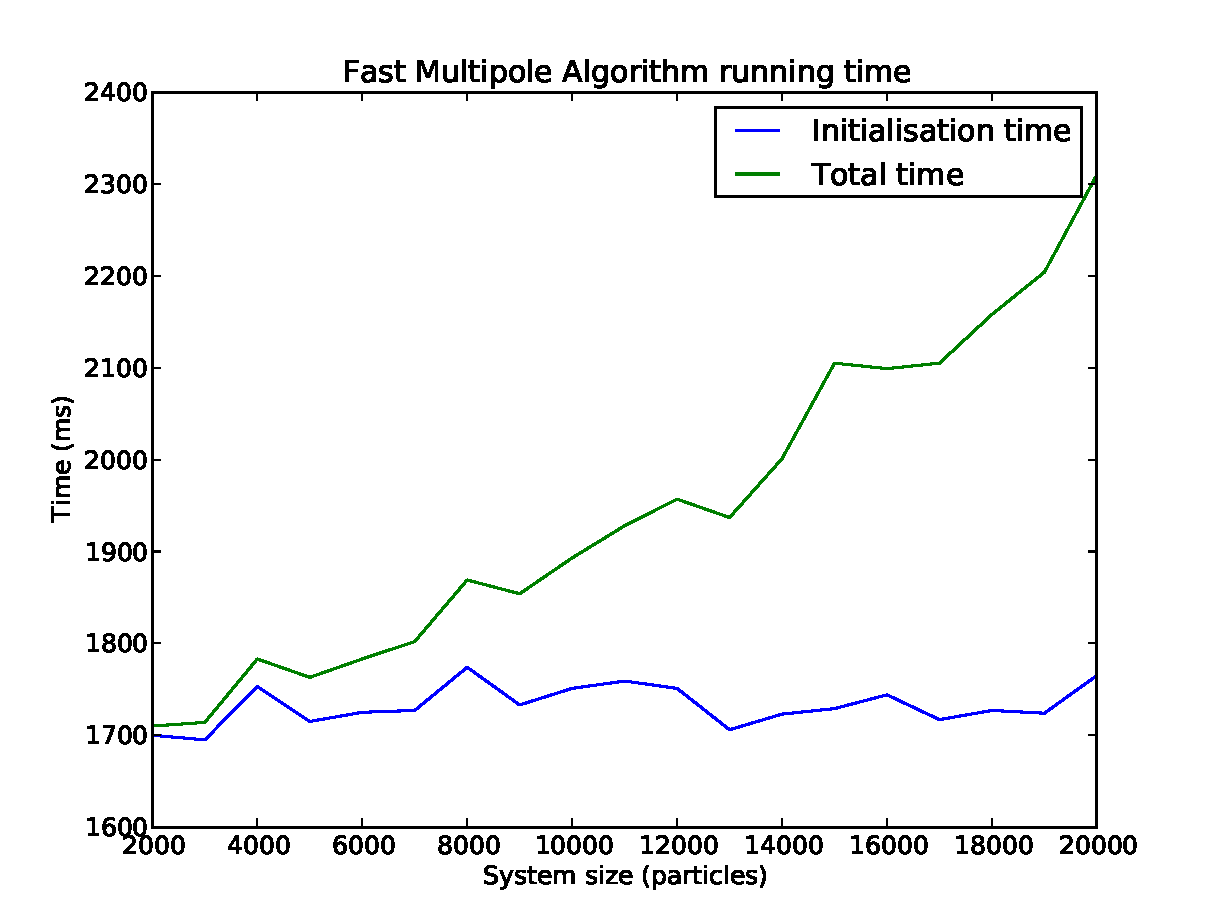
\includegraphics[width=\textwidth]{fma_2k_20k.pdf} \ecen
\end{frame}

\begin{frame}
\framesubtitle{Particle Mesh Ewald Algorithm}
\frametitle{Particle Mesh Ewald complexity}
\bcen 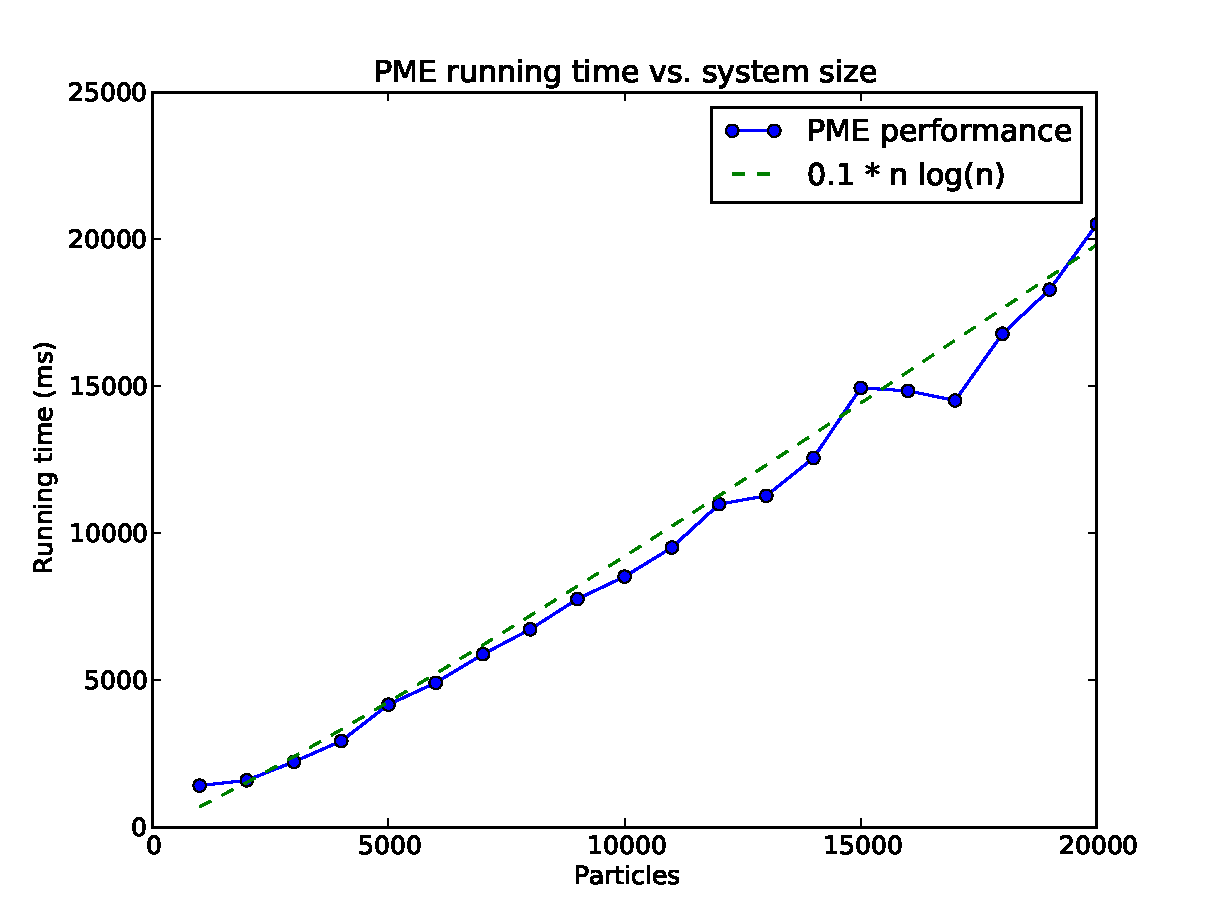
\includegraphics[width=\textwidth]{pme_algo_complex.pdf} \ecen
\end{frame}

\begin{frame}
\framesubtitle{Comparison}
\frametitle{Overlayed comparison graph}
\bcen 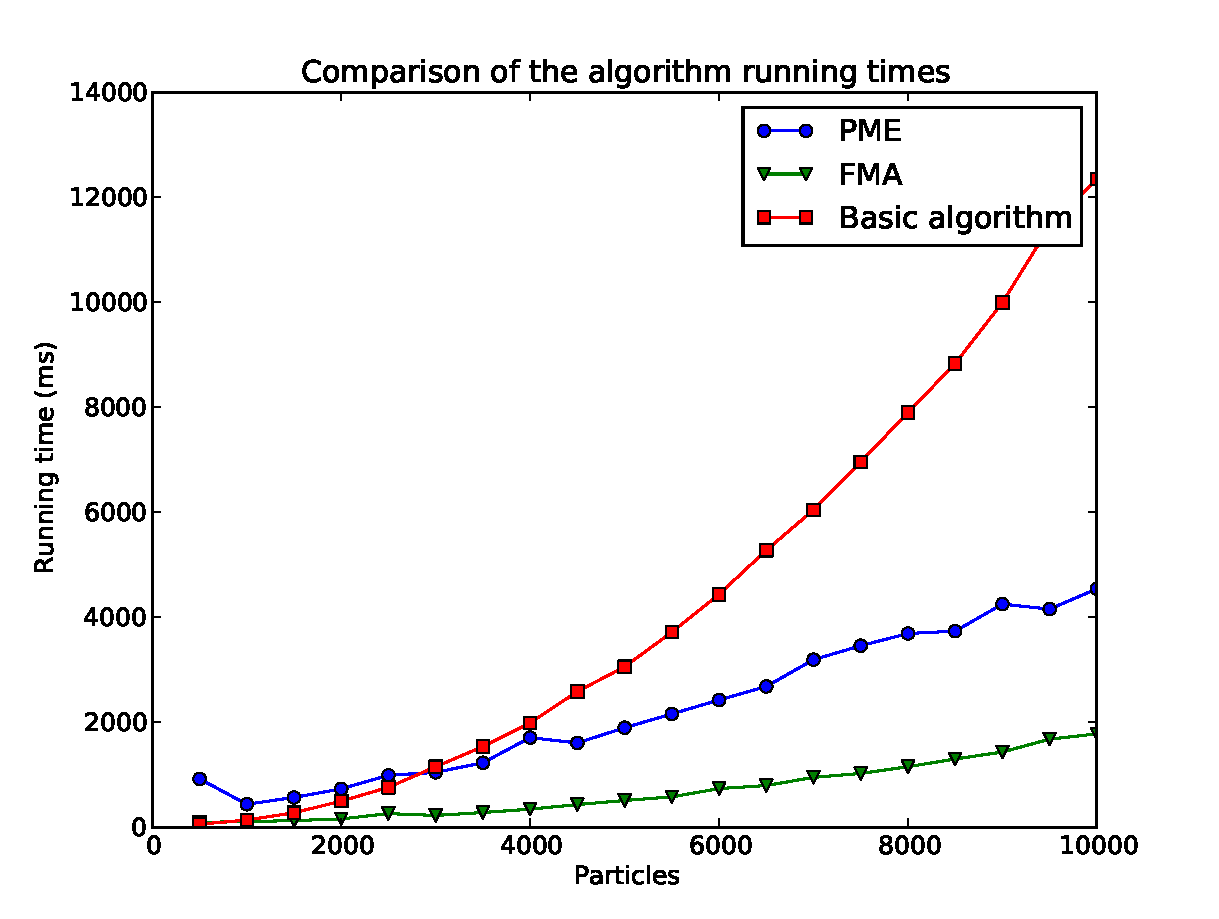
\includegraphics[width=\textwidth]{comp_graph.pdf} \ecen
\end{frame}

\begin{frame}
\framesubtitle{Comparison}
\frametitle{Overlayed comparison graph}
\bcen 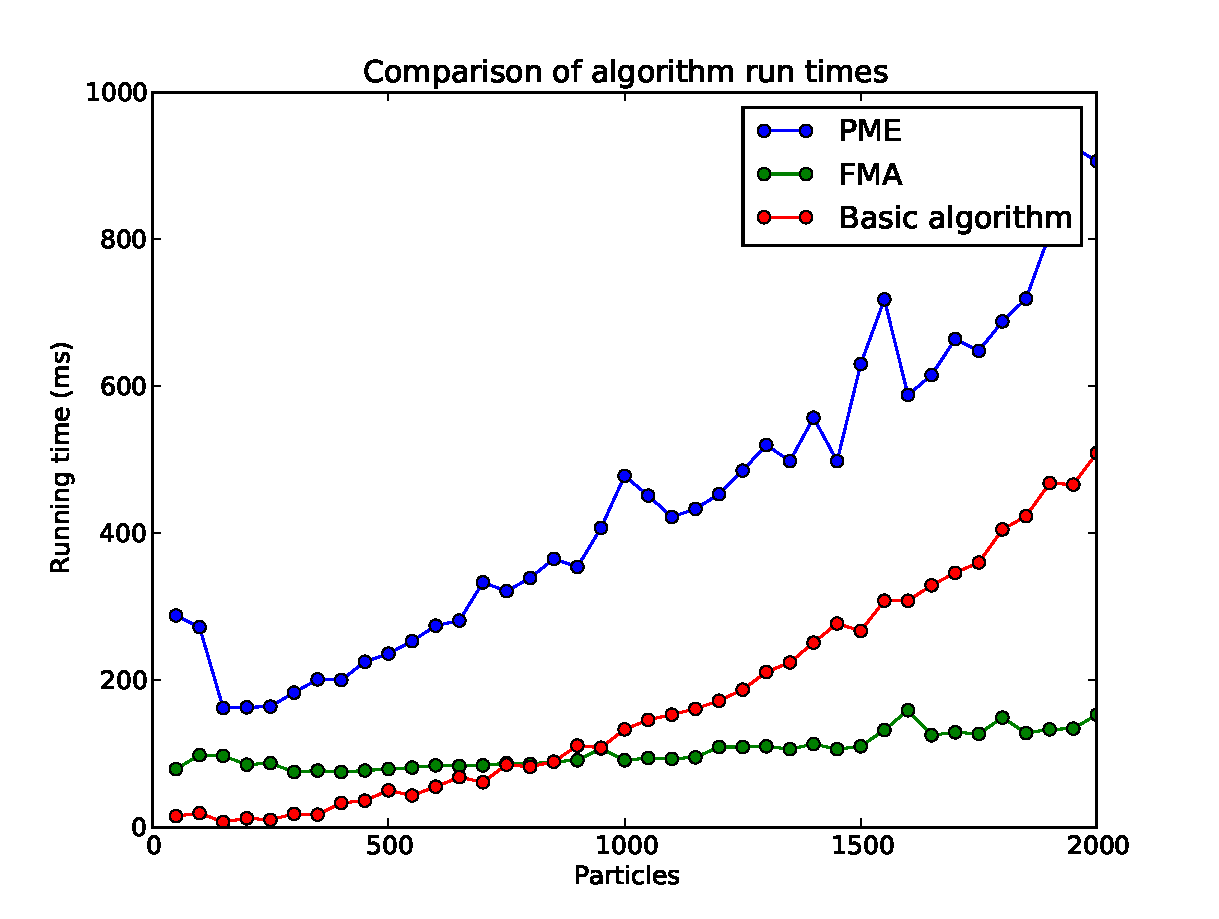
\includegraphics[width=\textwidth]{comp_graph_low.pdf} \ecen
\end{frame}

\section{Conclusion}
\begin{frame}
\frametitle{Conclusion}
\framesubtitle{Methods}
\begin{itemize}
\item<1-> Fast Multipole Algorithm is the fastest with the lowest run times over most cases
\item<2-> Particle Mesh Ewald has desriable features and more potential for paralellisation and optimisation
\item<3-> The Basic solution is not feasible for very large system sizes
\end{itemize}
\end{frame}

\begin{frame}
\frametitle{Conclusion}
\framesubtitle{Contributions}
\begin{itemize}
\item<1-> Created fucntional implementations of the Basic, Particle Mesh Ewald, and Fast Multipole algorithms in Java. 
\item<2-> Well documented and coded with readability in mind
\item<3-> Actualization of often abstractly defined algorithms
\item<4-> Complexity analysis of algorithms, crossover points found.
\item<5-> Bridged the gap between mathematicians, computer scientists, and computational chemists.
\end{itemize}
\end{frame}
\end{document}